\section{Biokompatibilität}
Verschiedene Materialien werden auf ihren Einfluss auf Hefekulturen hin untersucht. 
\begin{figure}[h!]
    \centering
    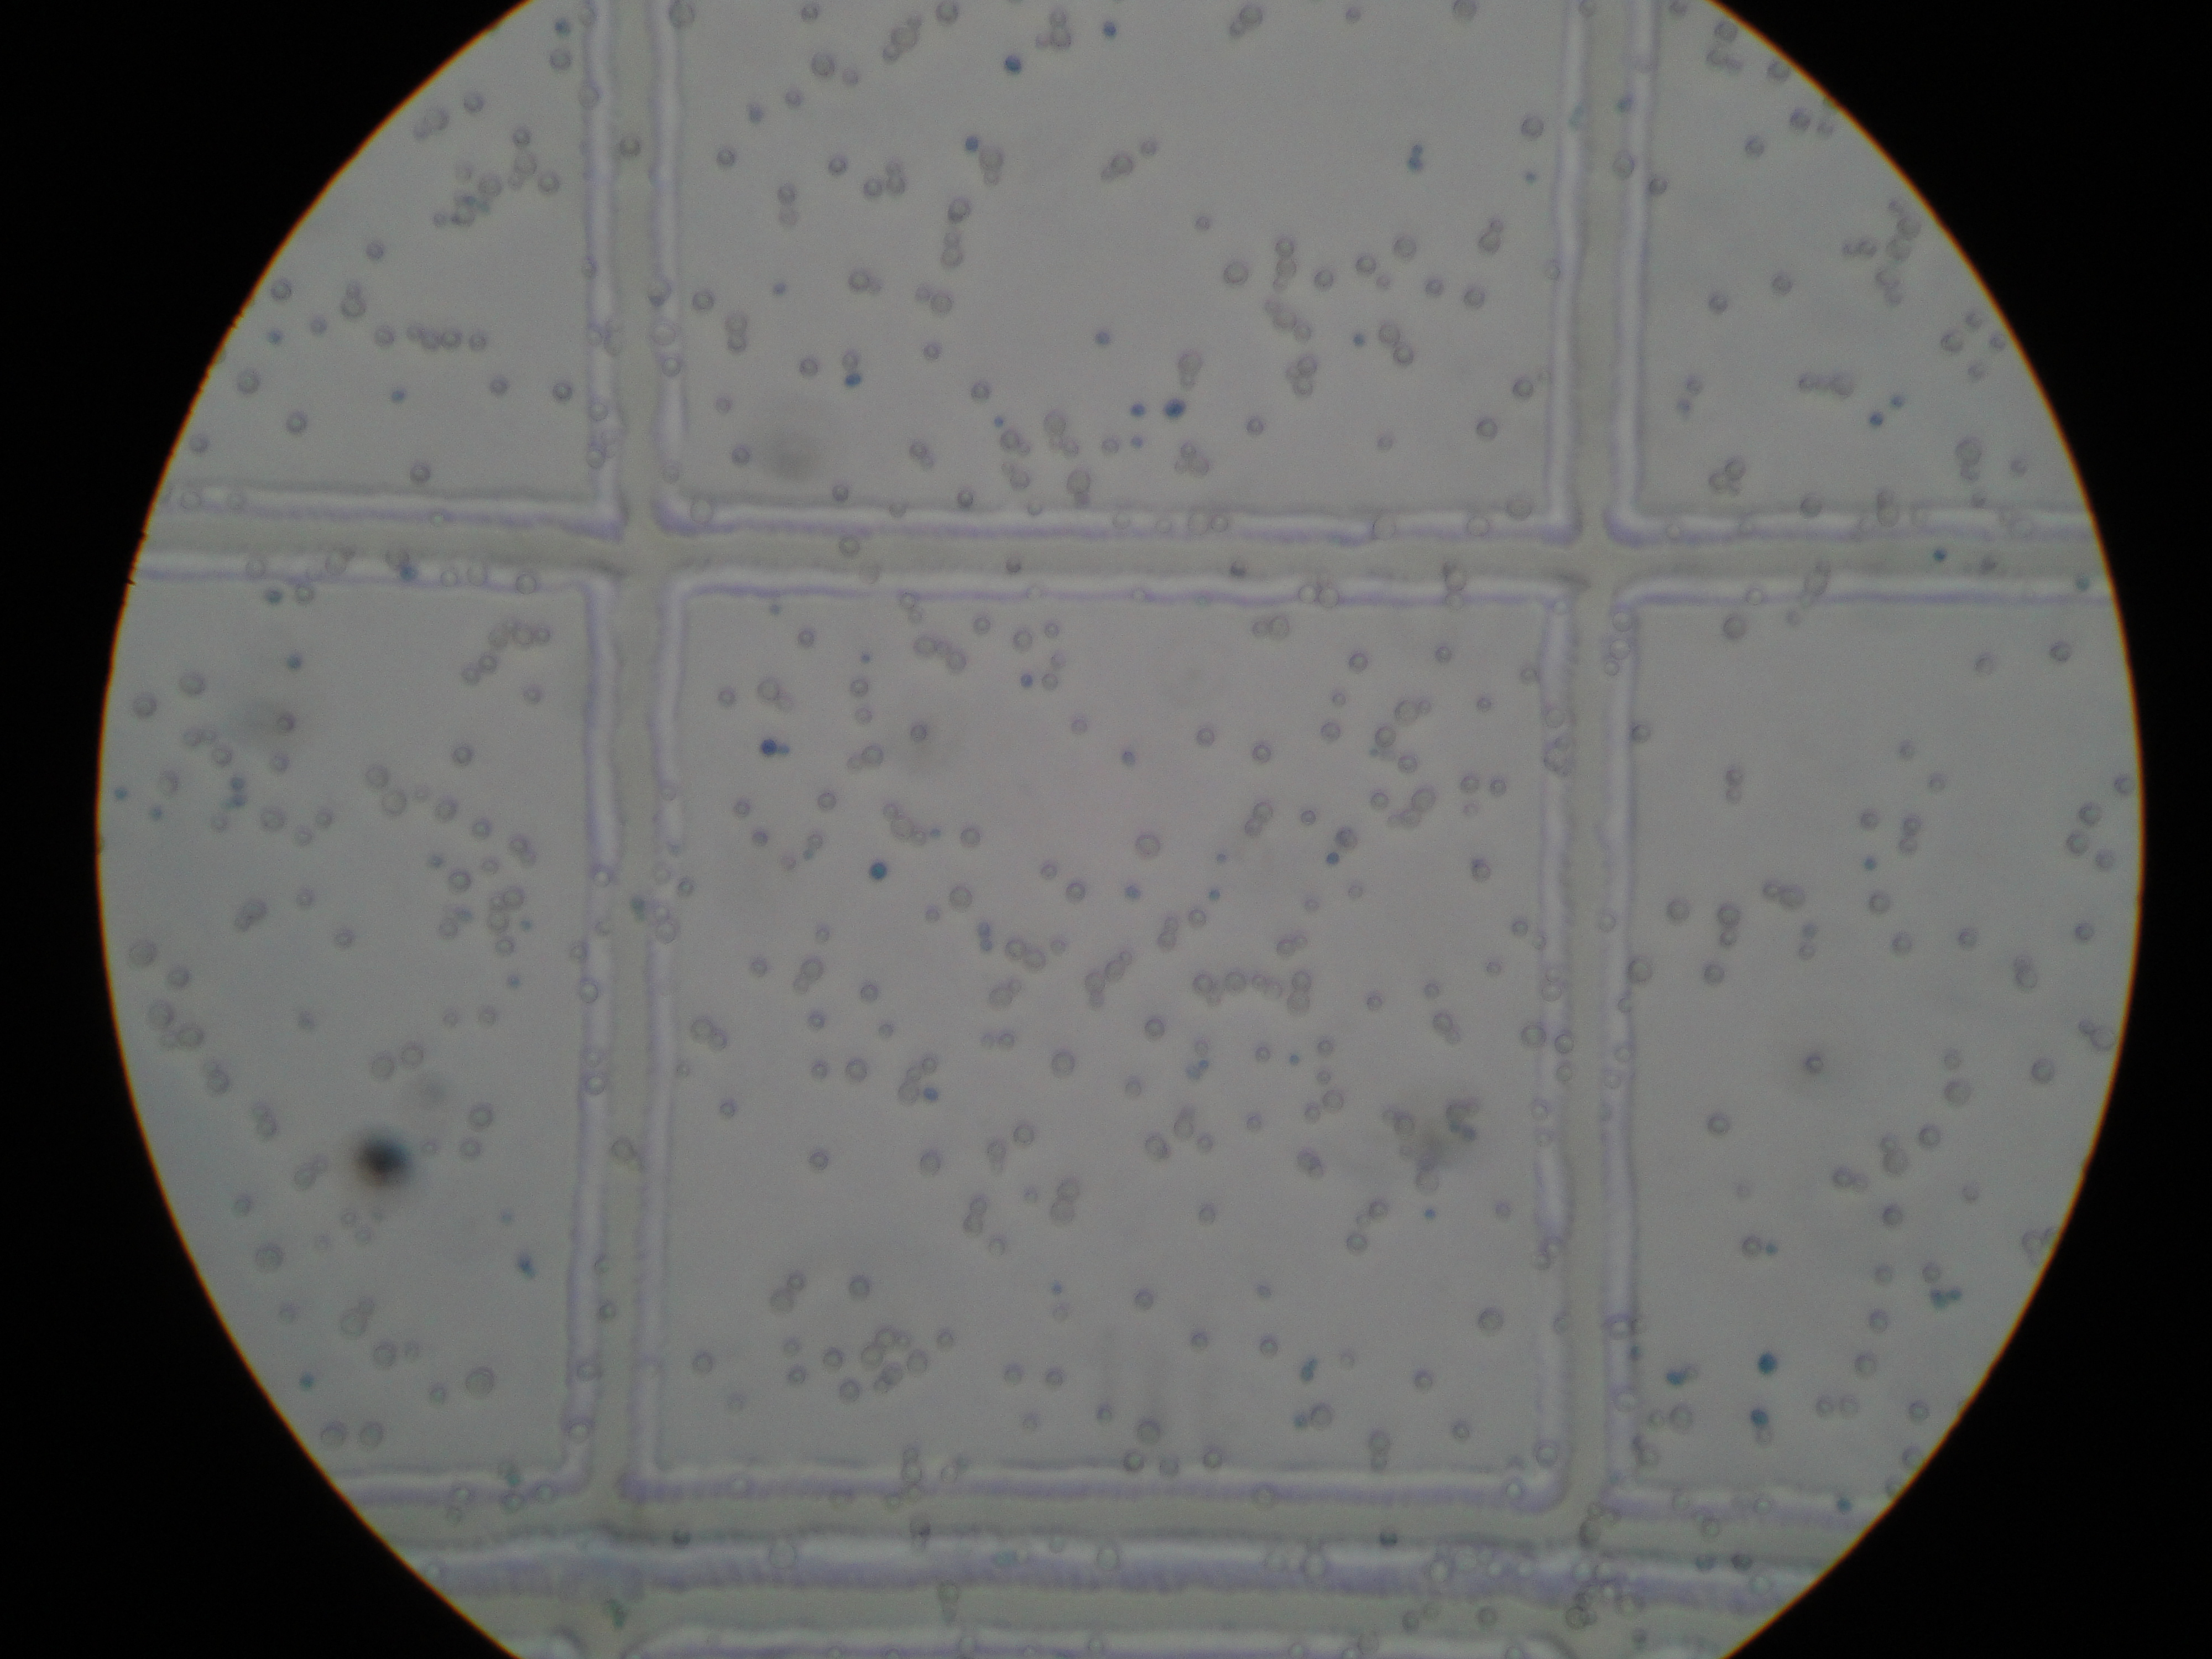
\includegraphics[width=0.5\textwidth]{fig/DSC02827.JPG}
    \caption{\matA}
    \label{fig:matA}
\end{figure}
\begin{figure}[h!]
    \centering
    \includegraphics[width=0.5\textwidth]{fig/DSC02830.JPG}
    \caption{\matB}
    \label{fig:matB}
\end{figure}
\begin{figure}[h!]
    \centering
    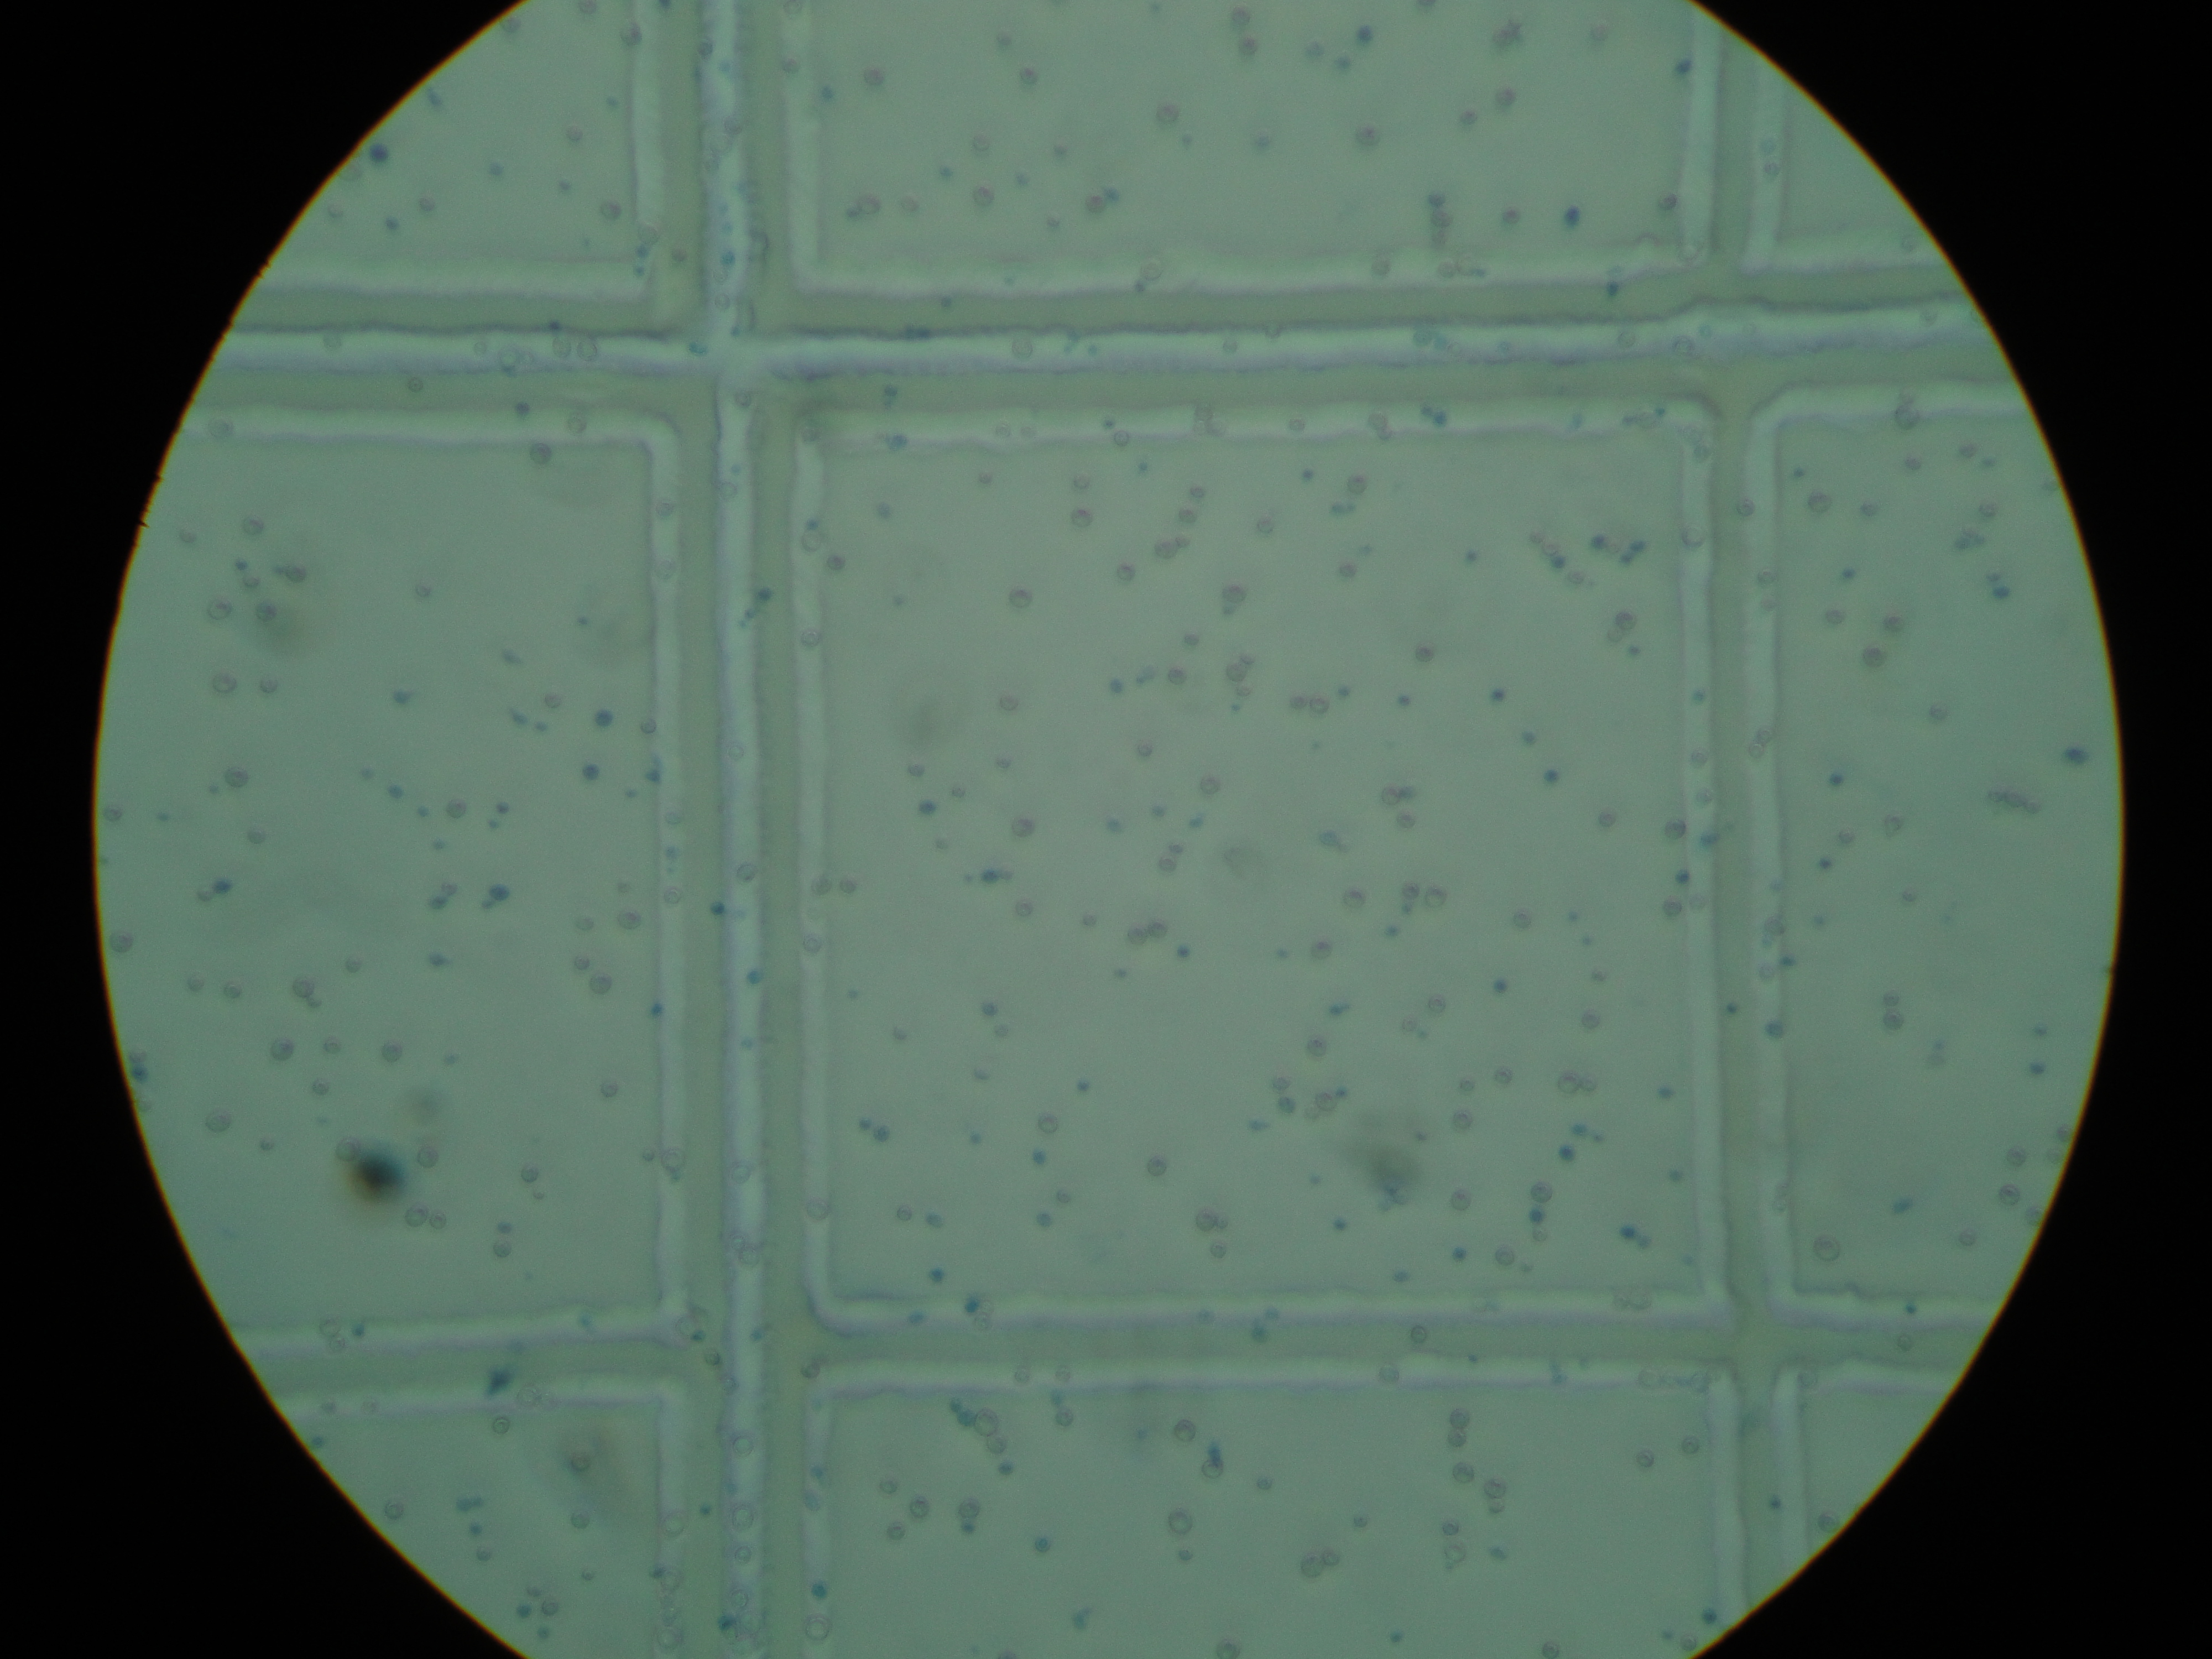
\includegraphics[width=0.5\textwidth]{fig/DSC02831.JPG}
    \caption{\matC}
    \label{fig:matC}
\end{figure}
\begin{figure}[h!]
    \centering
    \includegraphics[width=0.5\textwidth]{fig/DSC02832.JPG}
    \caption{\matD}
    \label{fig:matD}
\end{figure}
\begin{figure}[h!]
    \centering
    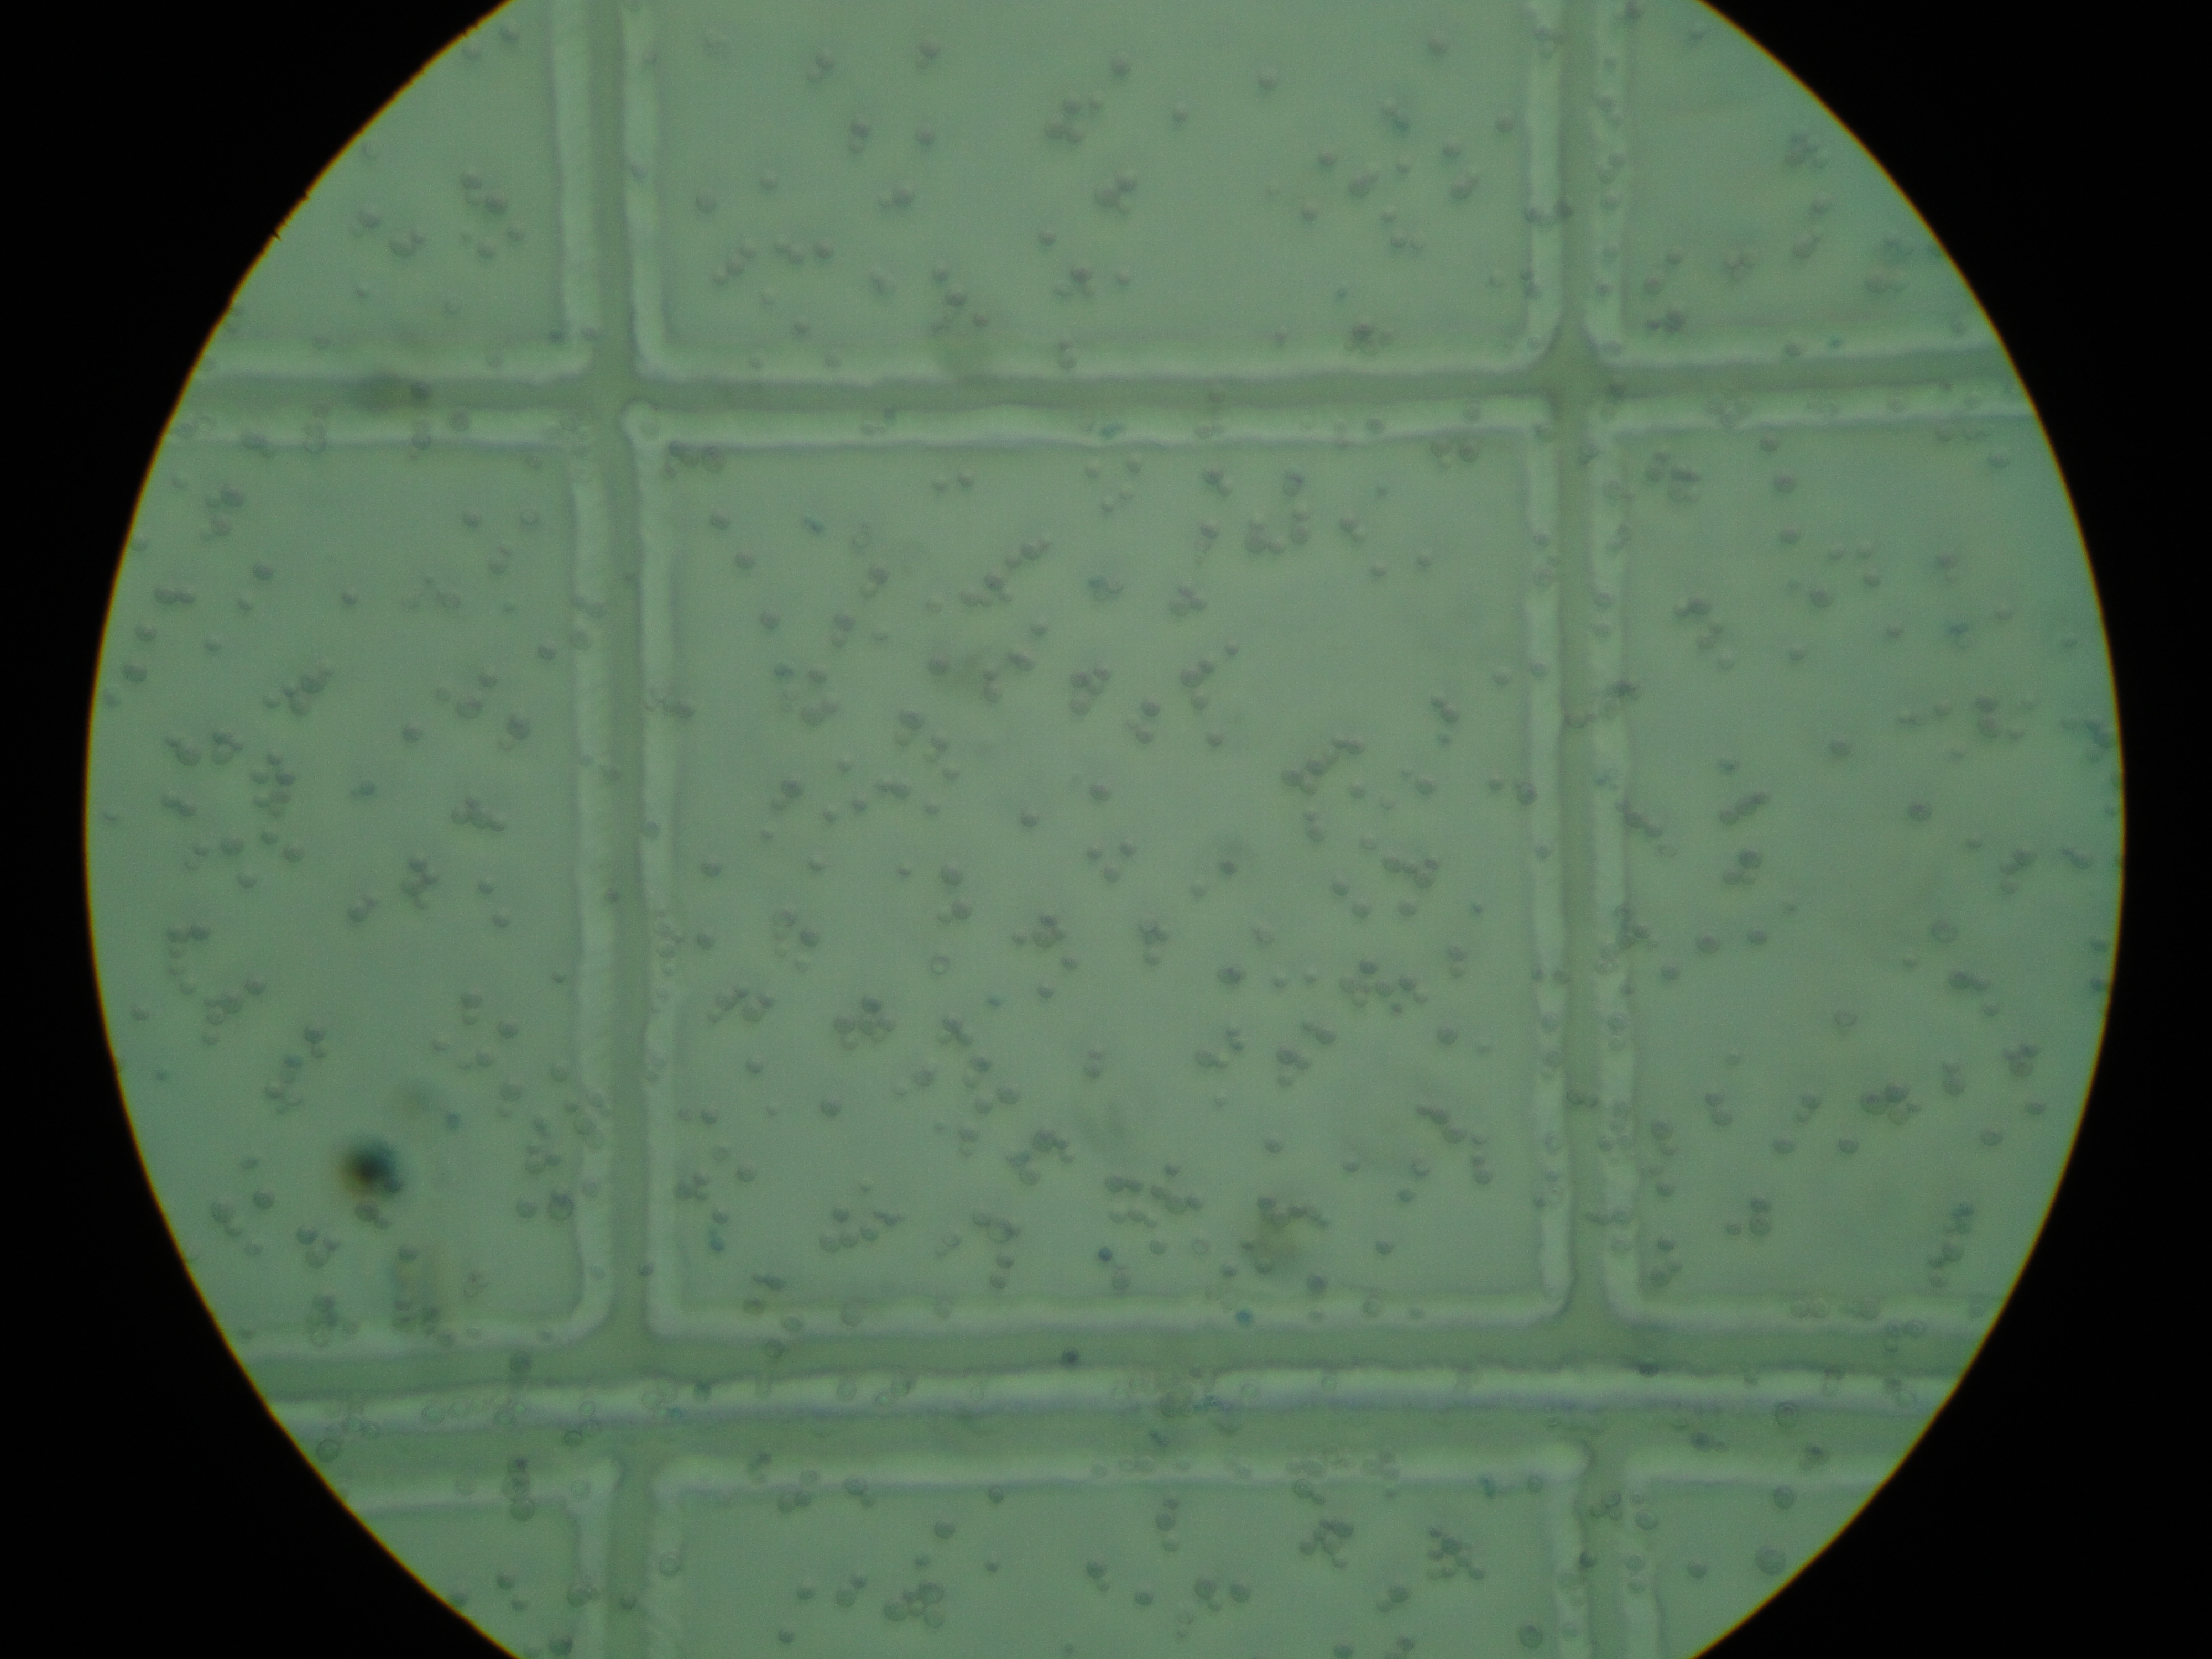
\includegraphics[width=0.5\textwidth]{fig/DSC02833.JPG}
    \caption{\matE}
    \label{fig:matE}
\end{figure}
\FloatBarrier
%\clearpage
\begin{table}[h!]
    \centering
    \begin{zebratabular}{lccr}
        \rowcolor{gray} Material & Lebende Zellen & Tote Zellen & Anteil tote Zellen \\
        \matA & 202 & 12 & 5.6\% \\
        \matB &  76 & 29 & 27.6\% \\
        \matC & 122 & 38 & 23.8\% \\
        \matD & 132 &  0 & 0\% \\
        \matE & 281 & 24 & 7.87\% \\
    \end{zebratabular}
    \caption{Auswertung}
\end{table}
